\documentclass[preprint,12pt,aps,pra,showkeys,amsmath,amssymb,superscriptaddress,floatfix]{revtex4-2}
\usepackage[T1]{fontenc}
\usepackage[utf8]{inputenc}
\usepackage{amsmath,amssymb,amsthm,mathtools,mathrsfs}
\usepackage{microtype,booktabs,enumitem}
\usepackage{xcolor,tikz,etoolbox}
\usepackage[skins,breakable]{tcolorbox}
\usepackage{needspace}
% Keep diagram geometry independent of REVTeX preprint body spacing.
\AtBeginEnvironment{tikzpicture}{\linespread{1}\selectfont}
\usetikzlibrary{arrows.meta,positioning,calc,fit,decorations.pathreplacing}
\usepackage{graphicx}
\usepackage{hyperref}

\definecolor{MMBlue}{RGB}{0,82,155}
\definecolor{MMOrange}{RGB}{200,80,0}
\tikzset{
 mmnode/.style={draw=MMBlue,rounded corners=2pt,fill=MMBlue!4,align=left,execute at begin node={\raggedright},text width=5cm,font=\fontsize{10}{12}\selectfont,inner sep=6pt},
 mmimport/.style={mmnode,draw=black!65,fill=black!4},
 mmcandidate/.style={mmnode,draw=MMOrange,dashed,fill=MMOrange!5},
 mmrejected/.style={mmnode,draw=black,densely dotted,fill=black!8},
 mmproof/.style={->,thick,MMBlue},
 mmflow/.style={->,semithick,black!70},
 mmrepair/.style={->,dashed,thick,MMOrange},
 mmcandidatearrow/.style={->,dashed,semithick,MMOrange},
 mmnote/.style={font=\scriptsize,fill=white,inner sep=2pt,align=center}}

\usepackage[section]{placeins}
\setlength{\emergencystretch}{3em}
\setlist{itemsep=3pt,topsep=4pt}
\newtheorem{theorem}{Theorem}[section]
\newtheorem{proposition}[theorem]{Proposition}
\newtheorem{lemma}[theorem]{Lemma}
\newtheorem{corollary}[theorem]{Corollary}
\theoremstyle{definition}
\newtheorem{definition}[theorem]{Definition}
\newtheorem{example}[theorem]{Example}
\theoremstyle{remark}
\newtheorem{remark}[theorem]{Remark}
% Avoid isolated statement headings and single-line paragraph fragments.
\BeforeBeginEnvironment{theorem}{\Needspace{6\baselineskip}}
\BeforeBeginEnvironment{definition}{\Needspace{5\baselineskip}}
\BeforeBeginEnvironment{proposition}{\Needspace{5\baselineskip}}
\BeforeBeginEnvironment{lemma}{\Needspace{5\baselineskip}}
\BeforeBeginEnvironment{corollary}{\Needspace{5\baselineskip}}
\clubpenalty=5000
\widowpenalty=5000
\newcommand{\R}{\mathbb R}\newcommand{\Z}{\mathbb Z}\newcommand{\N}{\mathbb N}
\newcommand{\Pa}{\operatorname{Pa}}\newcommand{\Desc}{\operatorname{Desc}}
\newcommand{\cl}{\operatorname{cl}}\newcommand{\cost}{\operatorname{cost}}
\newcommand{\status}{\operatorname{status}}
% Faculty cards: a visual rail groups the five faculties within one agent.
% The rail has no arrowhead and does not represent a proof dependency.
\newcommand{\mmfacultybadge}[1]{%
 \node[circle,draw=MMBlue,line width=1pt,fill=white,
 minimum size=7mm,inner sep=0pt,font=\sffamily\small\bfseries,text=MMBlue]
 at ([xshift=15pt,yshift=-15pt]frame.north west) {#1};}
\newcommand{\mmfacultyrail}{%
 \draw[MMBlue!80,line width=1pt]
 ([xshift=15pt,yshift=2pt]frame.north west)--
 ([xshift=15pt,yshift=-2pt]frame.south west);}
\newtcolorbox{mmfacultybox}[2]{enhanced,breakable,
 colback=MMBlue!4,colframe=MMBlue!4,boxrule=0pt,arc=3pt,
 left=39pt,right=9pt,top=4pt,bottom=4pt,
 before skip=2pt,after skip=2pt,
 fontupper=\small\linespread{1.1}\selectfont,
 overlay unbroken={\mmfacultyrail\mmfacultybadge{#1}},
 overlay first={\mmfacultyrail\mmfacultybadge{#1}},
 overlay middle={\mmfacultyrail},overlay last={\mmfacultyrail}}
\newcommand{\mmfaculty}[3]{%
 \begin{mmfacultybox}{#1}{#2}
 {\sffamily\bfseries\color{MMBlue}#2}\par\smallskip #3
 \end{mmfacultybox}}
\newcommand{\agent}[9]{%
 \Needspace{8\baselineskip}
 \subsubsection{#1}
 \noindent\textbf{Object.} #2\par
 \noindent\textbf{Role.} #3\par\smallskip
 \mmfaculty{E}{Ego}{#4}
 \mmfaculty{M}{Memory}{#5}
 \mmfaculty{I}{Intellect}{#6}
 \mmfaculty{S}{Sense}{#7}
 \mmfaculty{A}{Action}{#8}
 \smallskip\noindent #9\par}

\usepackage{longtable,array,calc}
\providecommand{\tightlist}{\setlength{\itemsep}{2pt}\setlength{\parskip}{0pt}}
\makeatletter
\def\frontmatter@abstract@produce{\par\addvspace{\frontmatter@preabstractspace}%
\begingroup\prep@absbox\unvbox\absbox\post@absbox\endgroup
\addvspace{\frontmatter@postabstractspace}}
\makeatother
\newcommand{\field}[2]{\par\smallskip\noindent\textbf{#1.} #2\par}
\setlength{\emergencystretch}{5em}
\AtBeginEnvironment{verbatim}{\small\linespread{1.0}\selectfont}


\hypersetup{colorlinks=true,linkcolor=MMBlue,urlcolor=MMBlue,pdfauthor={Dibakar Sigdel}}

\begin{document}

\title{Hilbert Projection Theorem\\[4pt]\large An End-to-End Meta-Math Walkthrough}

\author{Dibakar Sigdel}

\affiliation{Mindverse Computing LLC, Lynnwood, WA 98087, USA}

\date{October 2026}

\begin{abstract}

A minimizing sequence need not converge merely because its distances
converge. The parallelogram identity converts near-minimality into the
missing Cauchy estimate. The report presents the target theorem,
declared imports, a dependency graph, five-faculty node contracts, a
continuous proof, a worked example, and a hypothesis-repair audit. It is
an authored mathematical exposition, not a deployed-agent transcript or
a formal proof-assistant certificate.

\end{abstract}\maketitle\linespread{1.12}\selectfont

\noindent\textbf{FA-02 / Functional Analysis and Measure Theory / Report v1}

\section{Target and import contract}

\begin{theorem}

Let \(H\) be a real or complex Hilbert space and \(M\subset H\) a closed
linear subspace. For each \(x\in H\) there exists a unique \(m\in M\)
minimizing \(\|x-m\|\). Moreover \(x-m\perp M\), and the map \(P_Mx=m\)
is linear with \(\|P_Mx\|\le\|x\|\). Inner products are linear in the
first variable.

\end{theorem}

\subsection{Foundations and permitted imports}

Use completeness of \(H\), the parallelogram identity, Cauchy--Schwarz,
and the polarization rules for a complex inner product. A closed
subspace contains limits of its convergent sequences. The infimum
property supplies a sequence approaching a finite infimum.

\clearpage\section{Node interaction workflow}

\begin{center}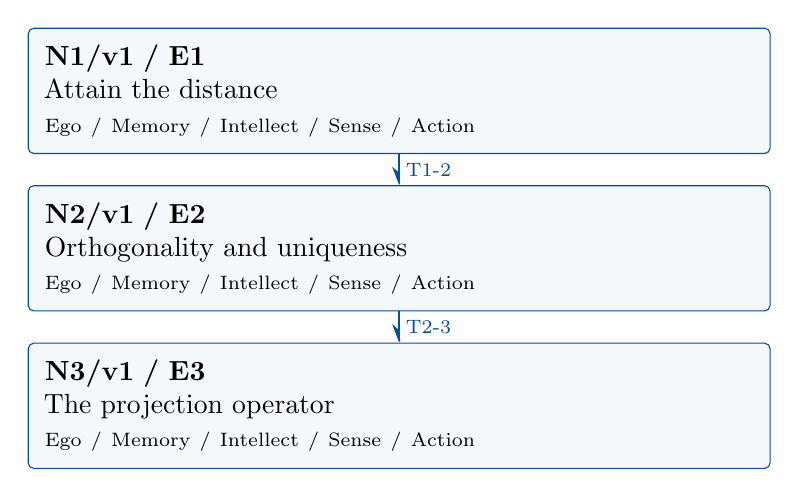
\begin{tikzpicture}[>=Stealth,x=1cm,y=1cm]

\node[mmnode,text width=9cm,minimum height=1.25cm] (N1) at (0,0.0) {\textbf{N1/v1 / E1}\\Attain the distance\\{\scriptsize Ego / Memory / Intellect / Sense / Action}};

\node[mmnode,text width=9cm,minimum height=1.25cm] (N2) at (0,-2.0) {\textbf{N2/v1 / E2}\\Orthogonality and uniqueness\\{\scriptsize Ego / Memory / Intellect / Sense / Action}};

\node[mmnode,text width=9cm,minimum height=1.25cm] (N3) at (0,-4.0) {\textbf{N3/v1 / E3}\\The projection operator\\{\scriptsize Ego / Memory / Intellect / Sense / Action}};

\draw[mmproof] (N1.south) -- node[mmnote,right] {T1-2} (N2.north);

\draw[mmproof] (N2.south) -- node[mmnote,right] {T2-3} (N3.north);

\end{tikzpicture}\end{center}

Each box is one mathematical agent containing all five faculties. Blue
arrows carry the versioned exports listed below. The layout gives a
reading order; only drawn arrows assert dependencies. Diagnostic repair
is separate from the proof DAG.

\subsection{Versioned evidence-transfer ledger}

\begingroup\small\linespread{1.05}\selectfont

\Needspace{5\baselineskip}\field{T1-2: N1/E1/v1 to N2}{There is \(m\in M\) with \(\|x-m\|=d\).}

\field{Receiving activity}{N2.1}

\field{Compatibility}{E1/v1, a minimizer \(m\), and each \(v\in M\). Check: In a complex
space, real variations alone only eliminate the real part of the inner
product.}

\Needspace{5\baselineskip}\field{T2-3: N2/E2/v1 to N3}{\(x-m\perp M\), and this condition characterizes the unique minimizer.}

\field{Receiving activity}{N3.1}

\field{Compatibility}{E2/v1 for every \(x\in H\). Check: The argument uses that \(M\) is a
linear subspace, not merely a closed set.}

\endgroup

\clearpage\section{Agent roles and five-faculty activities}\begingroup\small\linespread{1.05}\selectfont\setlist{itemsep=1pt,topsep=2pt}

\subsection{N1/v1: Attain the distance}

\field{Object and role}{Use the midpoint in the subspace to control differences of two
minimizing terms. \textbf{Local obligation:} There is \(m\in M\) with
\(\|x-m\|=d\).}

\field{Inputs}{\(d=\inf_{m\in M}\|x-m\|\) and a sequence \(m_n\in M\) with
\(\|x-m_n\|\to d\).}

\mmfaculty{E}{Ego}{Publish E1/v1 only after establishing this obligation: There is
\(m\in M\) with \(\|x-m\|=d\).}

\mmfaculty{M}{Memory}{\(d=\inf_{m\in M}\|x-m\|\) and a sequence \(m_n\in M\) with
\(\|x-m_n\|\to d\). Retain the stated assumptions and import versions.}

\mmfaculty{I}{Intellect}{Use the midpoint in the subspace to control differences of two
minimizing terms.}

\mmfaculty{S}{Sense}{The midpoint lies in \(M\); completeness gives a limit in \(H\) and
closedness places it in \(M\).}

\mmfaculty{A}{Action}{Carry out activities N1.1--N1.2 below, retaining each calculation and
construction as evidence.}

\smallskip\noindent\textbf{Numbered mathematical activities}

\begin{enumerate}[label=N1.\arabic*,leftmargin=3.4em]

\item Since \(0\in M\), \(0\le d\le\|x\|\). Choose \(m_n\) with
\(\|x-m_n\|<d+1/n\). The parallelogram identity gives
\(\|m_n-m_k\|^2=2\|x-m_n\|^2+2\|x-m_k\|^2-4\|x-(m_n+m_k)/2\|^2\). The
final squared norm is at least \(d^2\).

\item The resulting upper bound tends to zero as \(n,k\to\infty\). Thus
\((m_n)\) is Cauchy and converges in \(H\) to some \(m\). Closedness
gives \(m\in M\), and continuity of the norm gives \(\|x-m\|=d\).

\end{enumerate}

\field{Export E1/v1}{There is \(m\in M\) with \(\|x-m\|=d\).}

\field{Acceptance gate}{The midpoint lies in \(M\); completeness gives a limit in \(H\) and
closedness places it in \(M\).}

\field{Targeted repair}{If the minimizing sequence is declared convergent without an estimate,
insert the parallelogram bound; if \(M\) is not closed, the original
attainment claim needs a changed hypothesis. Withhold this export and
recheck its descendants after a versioned correction.}

\clearpage

\subsection{N2/v1: Orthogonality and uniqueness}

\field{Object and role}{Vary the minimizer along real and imaginary scalar multiples of \(v\).
\textbf{Local obligation:} \(x-m\perp M\), and this condition
characterizes the unique minimizer.}

\field{Inputs}{E1/v1, a minimizer \(m\), and each \(v\in M\). Incoming proof exports:
E1/v1 at N2.1.}

\mmfaculty{E}{Ego}{Publish E2/v1 only after establishing this obligation: \(x-m\perp M\),
and this condition characterizes the unique minimizer.}

\mmfaculty{M}{Memory}{E1/v1, a minimizer \(m\), and each \(v\in M\). Incoming proof exports:
E1/v1 at N2.1. Retain the stated assumptions and import versions.}

\mmfaculty{I}{Intellect}{Vary the minimizer along real and imaginary scalar multiples of \(v\).}

\mmfaculty{S}{Sense}{In a complex space, real variations alone only eliminate the real part
of the inner product.}

\mmfaculty{A}{Action}{Carry out activities N2.1--N2.2 below, retaining each calculation and
construction as evidence.}

\smallskip\noindent\textbf{Numbered mathematical activities}

\begin{enumerate}[label=N2.\arabic*,leftmargin=3.4em]

\item Write \(r=x-m\). For real \(t\), minimality implies
\(0\le\|r-tv\|^2-\|r\|^2=-2t\operatorname{Re}\langle r,v\rangle+t^2\|v\|^2\).
Taking small positive and negative \(t\) forces
\(\operatorname{Re}\langle r,v\rangle=0\). In the complex case repeat
with \(iv\) to get the imaginary part zero.

\item For any \(w\in M\), orthogonality gives \(\|x-w\|^2=\|r\|^2+\|m-w\|^2\).
Hence equality with the minimum holds only for \(w=m\). Conversely an
orthogonal residual gives this identity and therefore a minimizer.

\end{enumerate}

\field{Export E2/v1}{\(x-m\perp M\), and this condition characterizes the unique minimizer.}

\field{Acceptance gate}{In a complex space, real variations alone only eliminate the real part
of the inner product.}

\field{Targeted repair}{If only real orthogonality has been checked, add the \(iv\) variation
and revalidate uniqueness. Withhold this export and recheck its
descendants after a versioned correction.}

\clearpage

\subsection{N3/v1: The projection operator}

\field{Object and role}{Apply uniqueness of the orthogonal decomposition to sums and scalar
multiples. \textbf{Local obligation:} \(P_M\) is linear and contractive:
\(\|P_Mx\|\le\|x\|\).}

\field{Inputs}{E2/v1 for every \(x\in H\). Incoming proof exports: E2/v1 at N3.1.}

\mmfaculty{E}{Ego}{Publish E3/v1 only after establishing this obligation: \(P_M\) is linear
and contractive: \(\|P_Mx\|\le\|x\|\).}

\mmfaculty{M}{Memory}{E2/v1 for every \(x\in H\). Incoming proof exports: E2/v1 at N3.1.
Retain the stated assumptions and import versions.}

\mmfaculty{I}{Intellect}{Apply uniqueness of the orthogonal decomposition to sums and scalar
multiples.}

\mmfaculty{S}{Sense}{The argument uses that \(M\) is a linear subspace, not merely a closed
set.}

\mmfaculty{A}{Action}{Carry out activities N3.1--N3.2 below, retaining each calculation and
construction as evidence.}

\smallskip\noindent\textbf{Numbered mathematical activities}

\begin{enumerate}[label=N3.\arabic*,leftmargin=3.4em]

\item For \(x,y\in H\) and scalars \(a,b\), \(aP_Mx+bP_My\) lies in \(M\),
while \(a(x-P_Mx)+b(y-P_My)\) is orthogonal to \(M\). E2 identifies this
as the unique decomposition of \(ax+by\), proving linearity.

\item The decomposition \(x=P_Mx+(x-P_Mx)\) is orthogonal, so
\(\|x\|^2=\|P_Mx\|^2+\|x-P_Mx\|^2\). This proves the norm bound and
completes all assertions.

\end{enumerate}

\field{Export E3/v1}{\(P_M\) is linear and contractive: \(\|P_Mx\|\le\|x\|\).}

\field{Acceptance gate}{The argument uses that \(M\) is a linear subspace, not merely a closed
set.}

\field{Targeted repair}{If projection onto a nonlinear closed set is claimed linear, restore the
subspace contract; linearity is not part of the general convex
projection theorem. Withhold this export and recheck its descendants
after a versioned correction.}

\endgroup\clearpage\section{Continuous mathematical proof}\label{sec:proof}

\subsection{N1 --- Attain the distance}\label{n1-attain-the-distance}

\begin{enumerate}
\def\labelenumi{\arabic{enumi}.}
\item
  \textbf{N1.1.} Since \(0\in M\), \(0\le d\le\|x\|\). Choose \(m_n\)
  with \(\|x-m_n\|<d+1/n\). The parallelogram identity gives
  \(\|m_n-m_k\|^2=2\|x-m_n\|^2+2\|x-m_k\|^2-4\|x-(m_n+m_k)/2\|^2\). The
  final squared norm is at least \(d^2\).
\item
  \textbf{N1.2.} The resulting upper bound tends to zero as
  \(n,k\to\infty\). Thus \((m_n)\) is Cauchy and converges in \(H\) to
  some \(m\). Closedness gives \(m\in M\), and continuity of the norm
  gives \(\|x-m\|=d\).
\end{enumerate}

\subsection{N2 --- Orthogonality and
uniqueness}\label{n2-orthogonality-and-uniqueness}

\begin{enumerate}
\def\labelenumi{\arabic{enumi}.}
\item
  \textbf{N2.1.} Write \(r=x-m\). For real \(t\), minimality implies
  \(0\le\|r-tv\|^2-\|r\|^2=-2t\operatorname{Re}\langle r,v\rangle+t^2\|v\|^2\).
  Taking small positive and negative \(t\) forces
  \(\operatorname{Re}\langle r,v\rangle=0\). In the complex case repeat
  with \(iv\) to get the imaginary part zero.
\item
  \textbf{N2.2.} For any \(w\in M\), orthogonality gives
  \(\|x-w\|^2=\|r\|^2+\|m-w\|^2\). Hence equality with the minimum holds
  only for \(w=m\). Conversely an orthogonal residual gives this
  identity and therefore a minimizer.
\end{enumerate}

\subsection{N3 --- The projection
operator}\label{n3-the-projection-operator}

\begin{enumerate}
\def\labelenumi{\arabic{enumi}.}
\item
  \textbf{N3.1.} For \(x,y\in H\) and scalars \(a,b\), \(aP_Mx+bP_My\)
  lies in \(M\), while \(a(x-P_Mx)+b(y-P_My)\) is orthogonal to \(M\).
  E2 identifies this as the unique decomposition of \(ax+by\), proving
  linearity.
\item
  \textbf{N3.2.} The decomposition \(x=P_Mx+(x-P_Mx)\) is orthogonal, so
  \(\|x\|^2=\|P_Mx\|^2+\|x-P_Mx\|^2\). This proves the norm bound and
  completes all assertions.
\end{enumerate}

\hfill$\square$

\section{Worked orchestration}

In \(\mathbb R^3\), let \(M=\{(a,b,0):a,b\in\mathbb R\}\) and
\(x=(2,-1,3)\). The candidate \(m=(2,-1,0)\) has residual \((0,0,3)\)
perpendicular to \(M\). For \((a,b,0)\) the squared distance is
\(9+(2-a)^2+(-1-b)^2\), certifying the unique minimizer and \(d=3\).

\subsection{Boundary and hypothesis audit}

Let \(H=\ell^2\) and \(M=c_{00}\), the finitely supported sequences. For
\(x=(1/n)_{n\ge1}\), truncations in \(M\) approach \(x\), so the infimum
distance is zero. It is not attained because \(x\notin M\). This
isolates closedness.

\section{Illustrative failure and repair}

The following is an authored diagnostic scenario. Changed assumptions
define a new contract; they do not retroactively prove the original
statement.

\subsection{Rejected argument, diagnosis, and correction}
\textbf{Rejected export (N1):} every subspace admits a closest point.
\textbf{Sense witness:} the \(c_{00}\) example above. \textbf{Memory
diagnosis:} closedness was dropped when moving from a limit in \(H\) to
membership in \(M\). \textbf{Repair:} keep the stated closed-subspace
hypothesis and explicitly invoke it in N1.2. This repairs the proof of
the stated theorem; extending it to all subspaces is false. N2 and N3
must consume the corrected membership export.

\subsection{Publication and reuse}
The corrected export retains its explicit assumptions. A hypothetical
revision receives a new version, and each consuming activity is
rechecked; this scenario is not a recorded runtime event. \textbf{Next
direction:} Construct orthogonal decompositions and then the
Hilbert-space representation of continuous linear functionals in FA-03.

\par\medskip\begingroup\small\linespread{1.0}\selectfont\noindent\textbf{Provenance.} This authored proof is complete relative to its declared imports. Reuse
each export with its assumptions, proof, and version. The original
Markdown remains available for comparison.
\par\endgroup

\par\smallskip\begingroup\small\linespread{1.0}\selectfont\noindent\textbf{Further reading.} \href{https://ocw.mit.edu/courses/18-102-introduction-to-functional-analysis-spring-2021/resources/lecture-notes/}{MIT
OpenCourseWare, Introduction to Functional Analysis: lecture notes}. See
the lectures on integration, Hilbert spaces, Baire category, and
Hahn--Banach.\par\endgroup

\end{document}
